\begin{figure*}
    \begin{tabular}{m{95mm}m{5cm}}
      \begin{lstlisting}[basicstyle=\small]
  ordered (
    Label "Short label"     describes TextEdit "Text 1"
    Label "Loooooong label" describes TextEdit "Text 2"
  )
      \end{lstlisting} &
      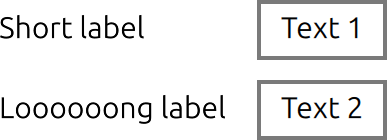
\includegraphics[scale=0.5]{Example1-Qt-QML.png} \\
      \hline\\
      \begin{lstlisting}[basicstyle=\small]
  ordered (
    Label "Looooong label" describes TextEdit "Text 1"
    Label "Medium label"   describes TextEdit "Text 2"
    Label "Short"          describes TextEdit "Text 3"
  )
      \end{lstlisting} &
      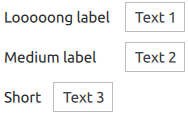
\includegraphics[scale=0.5]{Example2-Qt-QML.png} \\
      \hline
      \begin{lstlisting}[basicstyle=\small]
  ordered (
    Label "Short label"     describes TextEdit "Text 1"
    Label "Check box label" describes CheckBox _
    Label "Looooong label"  describes TextEdit "Text 2"
  )
      \end{lstlisting} &
      \vspace{1em}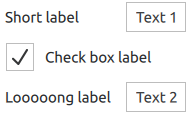
\includegraphics[scale=0.5]{Example4-Qt-QML.png} \\
      \hline\\
      \begin{lstlisting}[basicstyle=\small]
  ordered (
    Label "L 1"     describes CheckBox _
    Label "Lab 2"   describes CheckBox _
    Label "Label 3" describes CheckBox _
    Label "Label 4" describes CheckBox _
    Label "L 5"     describes CheckBox _
    Label "Lab 6"   describes CheckBox _
  )
      \end{lstlisting} &
      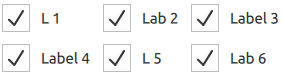
\includegraphics[scale=0.5]{Example5-Qt-QML.png} \\
    \end{tabular}
    \caption{Examples of structures (left) and synthesized layouts (right)\\
      w.r.t. JetBrains guidelines}
    \label{fig:evaluation}
  \end{figure*}
